To better understand the performance and limitations of the Spark Streaming architecture, we conducted a benchmark study of the system. We added instrumentation code that allowed us to track the timestamps of a subset of the input data as it flows through the system.

A synthetic workload was used for our performance testing on Spark Streaming.
This workload consists of an application that listens for a stream of text records.
The records have sizes between 15-25 bytes, and each holds a unique ID and a timestamp of time when the data was generated.
For each micro-batch, the application computes the difference between the current time and the time specified by the record, and use it to define the end-to-end latency of that record.

This workload only requires one stage per batch, since no aggregations are needed. As well, the work done by each task is very lightweight, since it only parses numbers and perform subtractions.
Despite the near-trivial computation, we believe that this application does is comparable with computations carried out on streaming systems. Due to latency constraints, fast streaming applications cannot be overly complex. They are likely to use filtering and simple aggregations, which are operations that can scale linearly with the resources available.
Also, often work can be completed more quickly with smart pipelining or different levels of parallelism, both of which are out of the scope of this paper. Our goal is to look at the code path that every workload uses, and identify and minimize the bottlenecks.


To run this benchmark, we first developed a record generator that can generate the type of workload described previously. Our record generator takes a record size and a data rate as input, listens on a socket for connections. For each incoming connection, it continuously generates as many records as needed to reach the specified data rate per second, until the connection or the generator is killed.

We deployed the generator and the Spark Streaming application on a dedicated cluster of machines, each equipped with a 16-core Intel Xeon CPU E5-1680 v2 @ 3.00GHz and 64GB of RAM. Each Receiver was run on a separate machine, and connected to a data generator for input.

\begin{figure}[t!]
  \begin{center}
    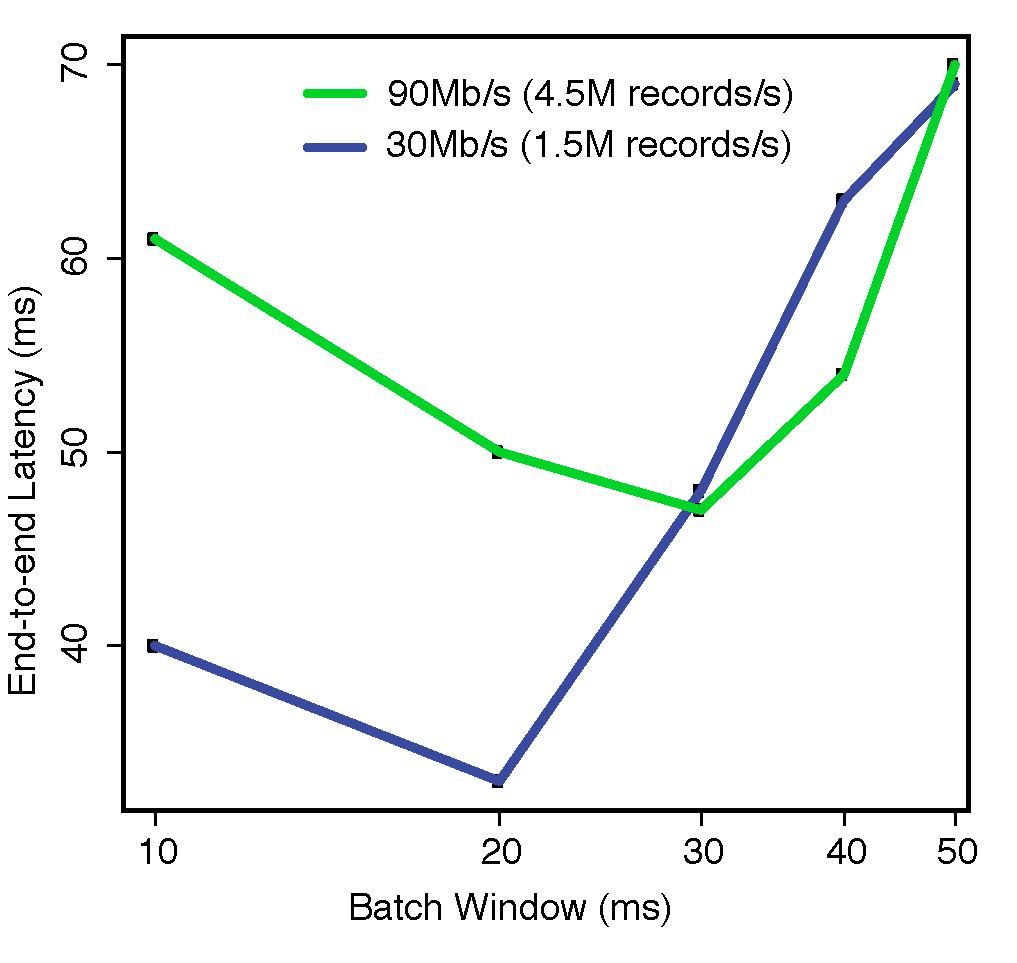
\includegraphics[scale=0.50]{images_graphs/batchsize_vs_latency/batchsize_vs_latency_illustrator.pdf}
  \end{center}
  \caption{Average end-to-end latency for different batch window sizes, different throughputs, and a fixed block interval of 2ms. For batch windows smaller than 10ms the average end-to-end latency tens to infinity.}
  \label{fig:Batchsize_vs_latency}
\end{figure}

\begin{figure}[t!]
  \begin{center}
    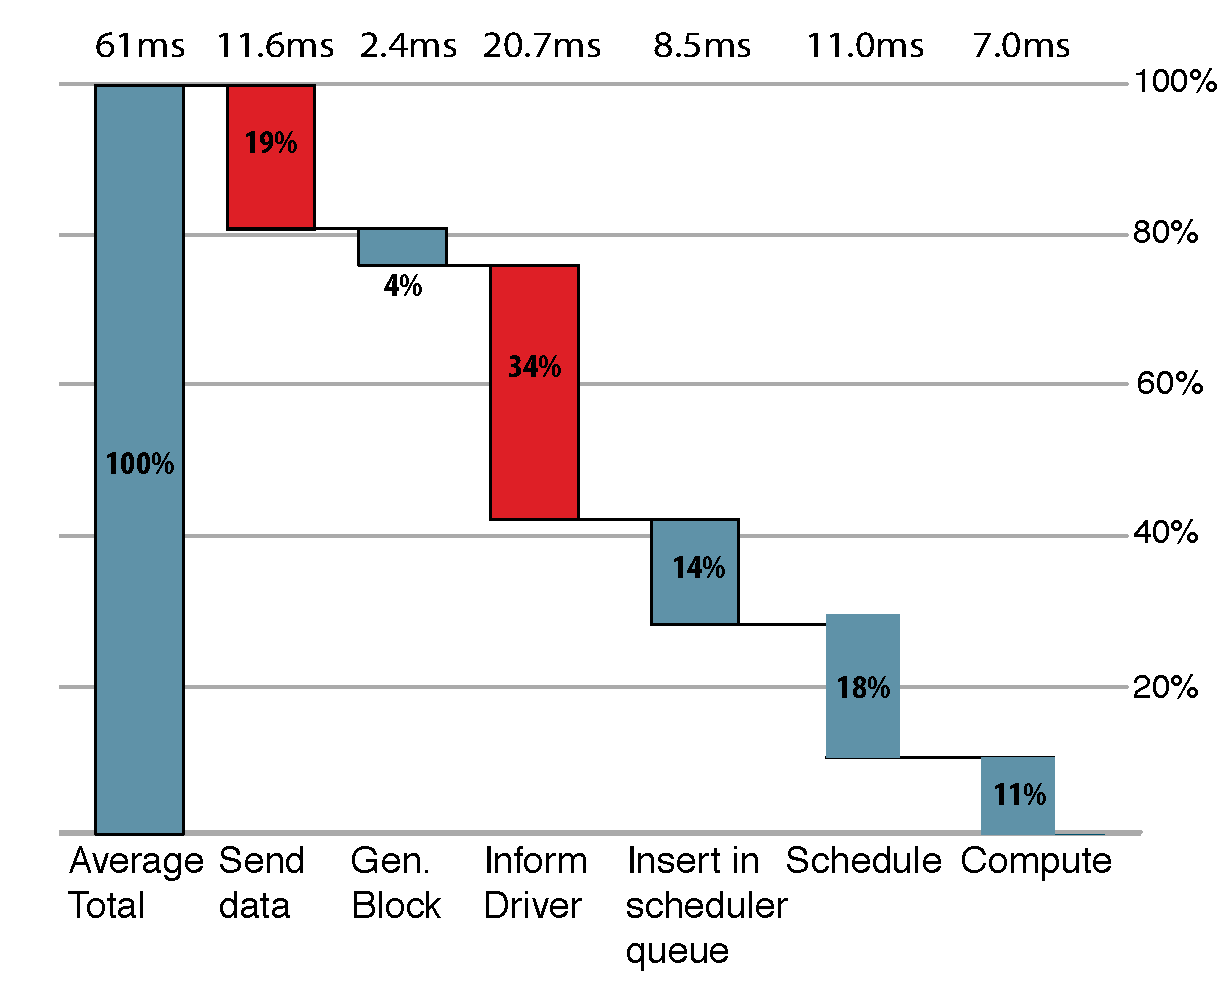
\includegraphics[scale=0.40]{images_graphs/waterfall/Rplots_illustrator.pdf}
  \end{center}
  \caption{Execution time breakdown for a batch window of 10ms at 90MB/s. The timestamp of the data is collected when 1) the data generator generates the record, 2) the Receiver receives the record, 3) the record is put inside a block, 4) the block is stored and communicated to the Driver, 5) the Driver puts the block metadata inside a batch, 6) the batch is scheduled, and 7) the record is processed by a task.}
  \label{fig:SparkStreaming_time_breakdown}
\end{figure}

\begin{figure}[t!]
  \begin{center}
    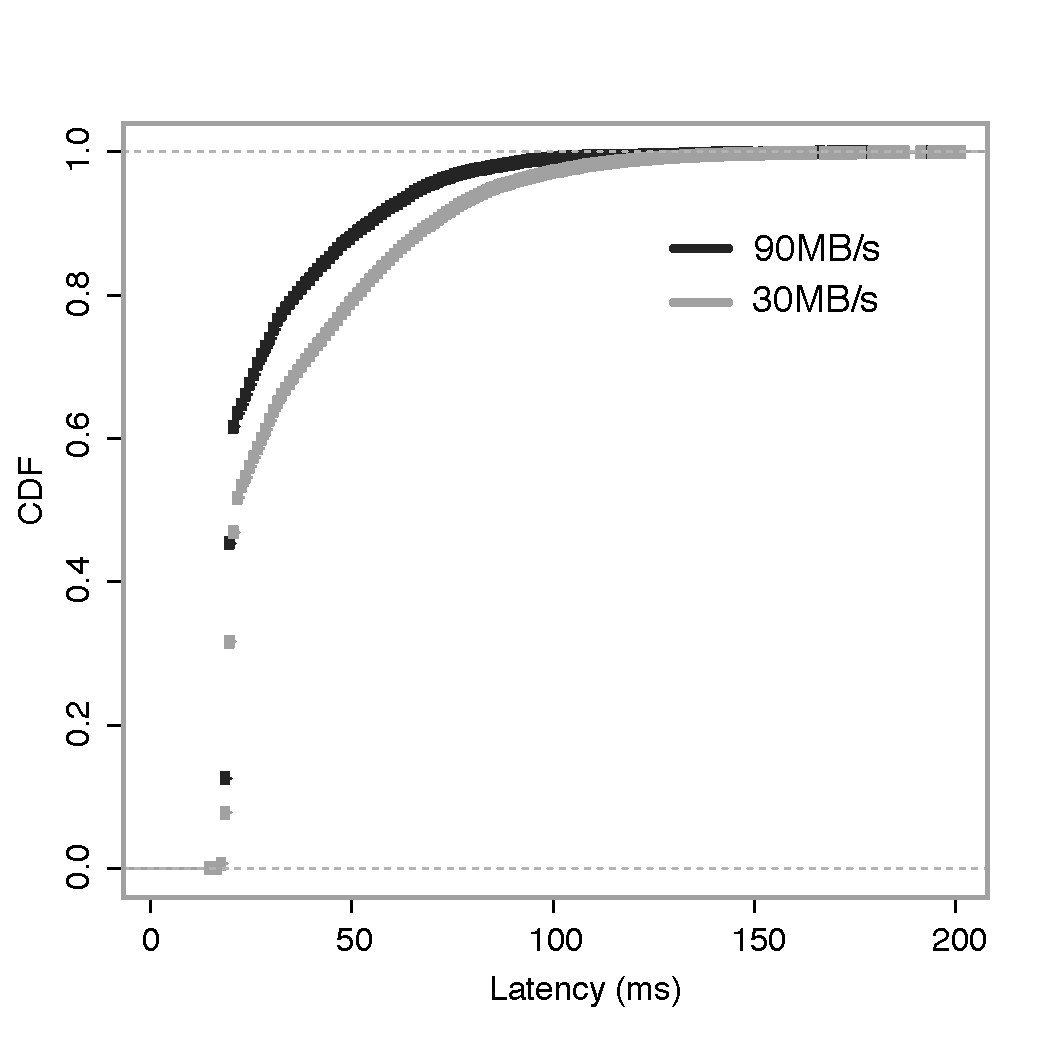
\includegraphics[scale=0.48]{images_graphs/cdf_latencies/cdf_e2e_times_illus.pdf}
  \end{center}
  \caption{CDF of latencies for a batch window of 10ms at 90MB/s and 30MB/s.}
  \label{fig:CDF_latencies}
\end{figure}

The results of our experiment are shown in Figure~\ref{fig:Batchsize_vs_latency}.
This graph displays the average end-to-end latency obtained when running Spark Streaming with five different batch window values and two different throughput levels.
Changing the batch window configuration allows us to tune the responsiveness of the system: a lower value means that each records on average spends less time in the Receiver, waiting to be put into a batch and subsequently processed by a task.
Varying the number of records generated by the stream source (throughput) allows us to understand how Spark behaves when it has to do more or less work per unit of time and how that affects latency.

As expected, as we instruct Spark Streaming to spawn tasks more frequently -- smaller batch window -- the average end-to-end latency time decreases.
However, at some point decreasing the batch window has a negative effect on the resulting latency.

We also find that as we increase the throughput, the end-to-end latency increases.
When analysing the reason, we determined that Spark Streaming's Receiver can be a source of slowdown.
For instance, we found that one Receiver is not able to receive more than roughly 30 MB/s, or 1.5M records/s.
This has to do with the fact that the Receiver receives and stores data in a sequential fashion within a single-threaded loop.
As a result, for batch windows less than 10ms we found the system to be unstable. 
Because Spark Streaming is not able to process records as quickly as the rate of arrival of new records, the end-to-end latency increases indefinitely.

Next, to understand where time is spent, we decomposed the execution time of Spark Streaming to different phases, based on our instrumentations.
We chose the top left point of Figure~\ref{fig:Batchsize_vs_latency}, i.e. batch window of 10ms and throughput of 90MB/s, and show the breakdown in Figure~\ref{fig:SparkStreaming_time_breakdown}. 
This graph provides several insights. 
First, at most 11\% of the execution time is useful time.
Second, roughly 20\% of the time is spent waiting for data to be transmitted from the source of the data to the Receiver.
This time has to do with the single-threaded loop design of reading tuples from the network.
Third, more than one third of the time is spent between generating a block of data and informing the driver about blocks received.
This time stems from the fact that the Receiver reserves one single thread to continuously store blocks and send the respective metadata to the Driver.
The approach does not seem to scale to workloads with a high number of blocks generated per unit of time.
Lastly, as expected, the time spent to schedule a micro-batch record is 11ms. Given a batch window of 10ms, each record will have to wait roughly 10ms to be scheduled.

Figure~\ref{fig:CDF_latencies} shows a CDF of the end-to-end latencies for different throughput levels. The graph shows that a considerably-sized tail of records is served with high latency, implying high variance in end-to-end latency.

One caveat is that the record we choose to track is always the first record in the first block of every batch. This means the record is one of the first records arrived for the batch, and among the ones that waited the longest. Therefore, the median end-to-end latencies for the shown data points should be the displayed latency minus half of block interval as well as batch interval.

Overall, e believe these results motivate the need for an architecture that can scale and adapt to bursts of data in order to consistently provide acceptable latencies.
